\section{Systematic Literature Review}

Guided by Kitchenham's SLR framework, this study carefully addressed review planning (defining research questions, developing a protocol), conducting (literature search, study selection, data extraction and quality assessment), and reporting \cite{Kitchenham}.

\begin{figure}[ht]
    \centering
    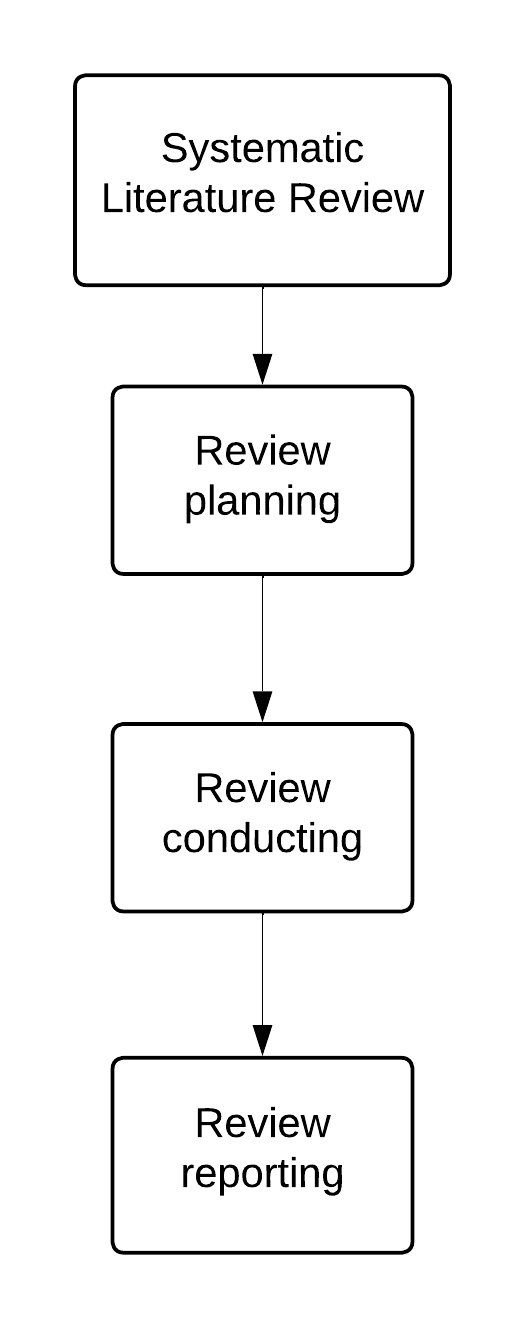
\includegraphics[width=0.3\linewidth]{figs/slr-overview.png}
    \caption{Systematic Literature Review process \cite{Kitchenham}}
    \label{fig:slr-overview}
\end{figure}

The figure \ref{fig:slr-overview} shows an overview of my work to execute a systematic literature review. I meticulously outlined a protocol and defined my overarching research questions 1 and 2. A comprehensive search strategy was then established to pinpoint pertinent articles within electronic databases relevant to the field of open source software motivation. Stringent inclusion and exclusion criteria ensured the selection of methodically sound studies. Following the search, I carefully screened titles and abstracts of retrieved database articles. Studies initially deemed relevant underwent a thorough full-text analysis. This systematic review will culminate in a detailed report encompassing search strategies, selection criteria, the number of articles evaluated at each stage, and an overarching synthesis of the findings.



\subsection{Review planning}

In chapter \ref{researchQuestions}, I explored the process of defining a research question. Here, I will concentrate on developing a protocol for the initial review planning phase of a \ac{slr}. While numerous scientific databases exist online, selecting the most suitable ones for evidence synthesis can be challenging \cite{academicSearchSystems}. This section will offer guidance on database selection and explain the rationale behind different choices.


% Web of Science and Scopus hold a strong reputation as the most reliable and comprehensive citation databases within the academic community \cite{zhu2020tale}. However, 

\subsubsection{Search criteria}
Building on a previous study from Chua and Zhang \cite{Chua_Zhang_2020}, I established inclusion criteria to ensure the selected articles addressed my research questions and utilized strong methodologies:

\begin{itemize}
    \item Research articles and conference papers, peer-reviewed and available through major academic search platforms like Google Scholar, Springer, \ac{ieee}, \ac{acm}, Science Direct.
    \item Restriction to English-language sources.
    \item Disciplines in Computer Science, Software Engineering
    \item Publication date: from 2000 to 2024.
    \item Specific search terms ("open source" OR "open source software") AND ("motivation" OR "contribution challenges" OR "social dynamics impact" OR "interest" OR "contribution barriers") within titles or descriptions.
    \item Prioritization of publications from leading information systems conferences and journals. Ex: ACM/IEEE International Conference on Software Engineering, IEEE Transactions on Software Engineering, Journal of Systems and Software,...
\end{itemize}

These search terms were employed to address the three research questions which are categorized in the table \ref{tab:categoriesSearchTerms}.

\begin{table}[ht]
    \centering
    \begin{tabular}{ | c | l | }
        \hline
        Category & Search terms                                   \\ \hline
        1        & OSS motivation and all synonyms                \\ \hline
        2        & Social dynamics impact on OSS and all synonyms \\  \hline
        3        & Contribution barriers of OSS and all synonyms  \\  \hline
    \end{tabular}
    \caption{Specific categories of search terms}
    \label{tab:categoriesSearchTerms}
\end{table}



\subsubsection{Data source}

To identify relevant literature, I executed the search strings across multiple databases. Each database was queried with the complete set of search strings, yielding varying results. In some instances, identical search strings produced an overabundance of results, while in others, they returned no results. Databases with no results were excluded from further analysis. The selected databases and their corresponding result counts are presented in the following table \ref{tab:initialSearch}.


\begin{table}[ht]
    \centering
    \begin{tabular}{ | l | c | c | c |}
        \hline
        Database       & Category 1      & Category 2     & Category 3      \\ \hline
        Google Scholar & 244 000 results & 17 800 results & 175 100 results \\ \hline
        Springer       & 623 results     & 161 results    & 327 results     \\ \hline
        IEEE           & 396 results     & 68 results     & 48 results      \\ \hline
        Science Direct & 4 200 results   & 97 results     & 15 results      \\ \hline
    \end{tabular}
    \caption{Initial search results from scientific databases}
    \label{tab:initialSearch}
\end{table}



\subsubsection{Inclusion and exclusion criteria}

To maintain a focused and methodologically review, I used inclusion and exclusion criteria to pinpoint studies aligned with my research questions. These criteria served as a consistent filter for all potential sources. The specific criteria are outlined below, and they were applied to every study retrieved from the selected databases.

Inclusion:
\begin{itemize}
    \item Accessible: The research paper must be accessible and downloadable either through LUT Academic Library or online database.
    \item Peer-Reviewed: The paper should be published in a reputable, peer-reviewed journal or conference proceedings. This ensures the quality and credibility of the research.
    \item Relevant to research questions: The paper must directly address the specific research questions at hand.
    \item Methodology transparency: The reasearch and data collection  methodologies must be metioned.
\end{itemize}

Exclusion:
\begin{itemize}
    \item Irrelevant content: Exclude papers that deviate significantly from my research questions or lack a clear connection to the area of study.
    \item Older papers (released before 2000) ought to be disregarded.
    \item Papers having fewer than four pages were removed.
    \item Papers cannot be accessed
    \item Papers were not written in English
    \item Papers topic were about open source but in hardware, economy, environment,... but not software
\end{itemize}

\subsubsection{Study selection}
A further procedures were taken for the final paper selection after applying the inclusion/exclusion criteria to each of the resultant papers.

\begin{itemize}
    \item Review the title, keyword, abstract, description for filtering
    \item Excluding duplicated studies.
    \item Ranking research papers by the number of times they've been cited and relevant to search term by search engine.
\end{itemize}


The initial search across various databases yielded approximately 500,000 potentially relevant papers. Due to resource constraints, the review process was limited to 50 papers per database. Following the application of inclusion and exclusion criteria, along with further selection procedures, a final set of 20 relevant and suitable articles was identified for this SLR. These papers are listed in table \ref{tab:databasePapers}, with full details provided in the Appendix \ref{App:A}. The paper selection process is displayed in the figure \ref{fig:paperselectionprocess}



\begin{figure}[ht]
    \centering
    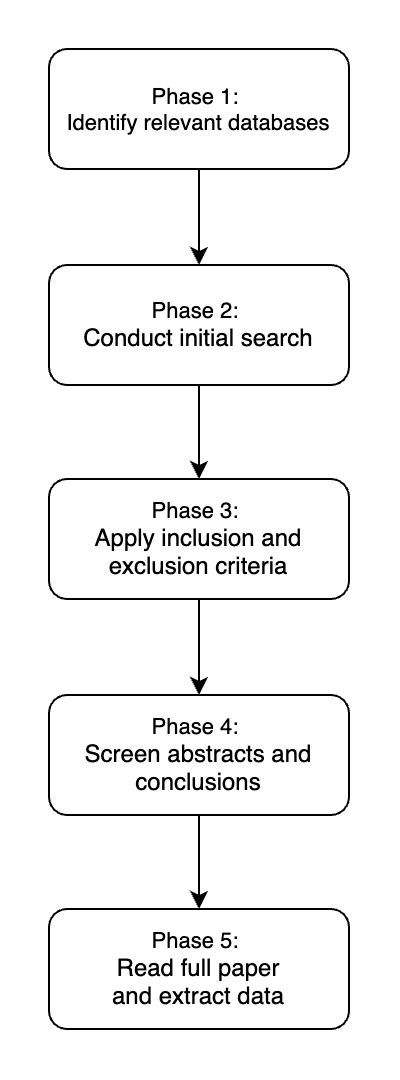
\includegraphics[width=0.3\linewidth]{figs/paperselectionprocess.png}
    \caption{Process of selecting papers for SLR}
    \label{fig:paperselectionprocess}
\end{figure}



\begin{table}[ht]
    \begin{tabular}{| m{7em} | m{5em}| m{18em} | }
        \hline
        Publisher                & Number of articles & Authors                                                                                                                                                                           \\ \hline
        Elsevier                 & 6                  & Bitzer, Schrettl \& Schröder (2007); Choi \& Pruett (2015); Li, Tan \& Teo (2012); Oreg \& Nov (2008); Steinmacher, Silva, Gerosa \& Redmiles (2015); Wu, Gerlach \& Young (2007) \\ \hline
        AISNET                   & 1                  & Ke \& Zhang, P. (2008)                                                                                                                                                            \\ \hline
        IEEE                     & 3                  & Ye \& Kishida (2003); Gerosa, Wiese, Trinkenreich, Link, Robles, Treude \& Sarma (2021); Zhang, Yuxia (2024)                                                                      \\ \hline
        ResearchGate             & 1                  & Zhao, Shengyu (2024)                                                                                                                                                              \\ \hline
        Springer                 & 3                  & Steinmacher, Conte, Gerosa \& Redmiles (2019); Fershtman \& Gandal  (2007); Hannemann \& Klamma (2013) ; Hannemann \& Klamma (2013)                                               \\ \hline
        ACM                      & 3                  & Steinmacher, Conte, Gerosa \& Redmiles (2015); Guizani, Chatterjee, Trinkenreich, May, Noa-Guevara, Russell \& Sarma (2021) ; Hannebauer \& Gruhn (2017)                          \\ \hline
        Informs                  & 1                  & Roberts, Hann \& Slaughter (2006)                                                                                                                                                 \\ \hline
        Taylor \& Francis Online & 1                  & Alexander Hars (2002)                                                                                                                                                             \\ \hline
        EASST                    & 1                  & Freeman (2007)                                                                                                                                                                    \\ \hline
    \end{tabular}
    \caption{Selected papers for SLR}
    \label{tab:databasePapers}
\end{table}


\begin{figure}[ht]
    \hspace*{-0.5in}
    \centering
    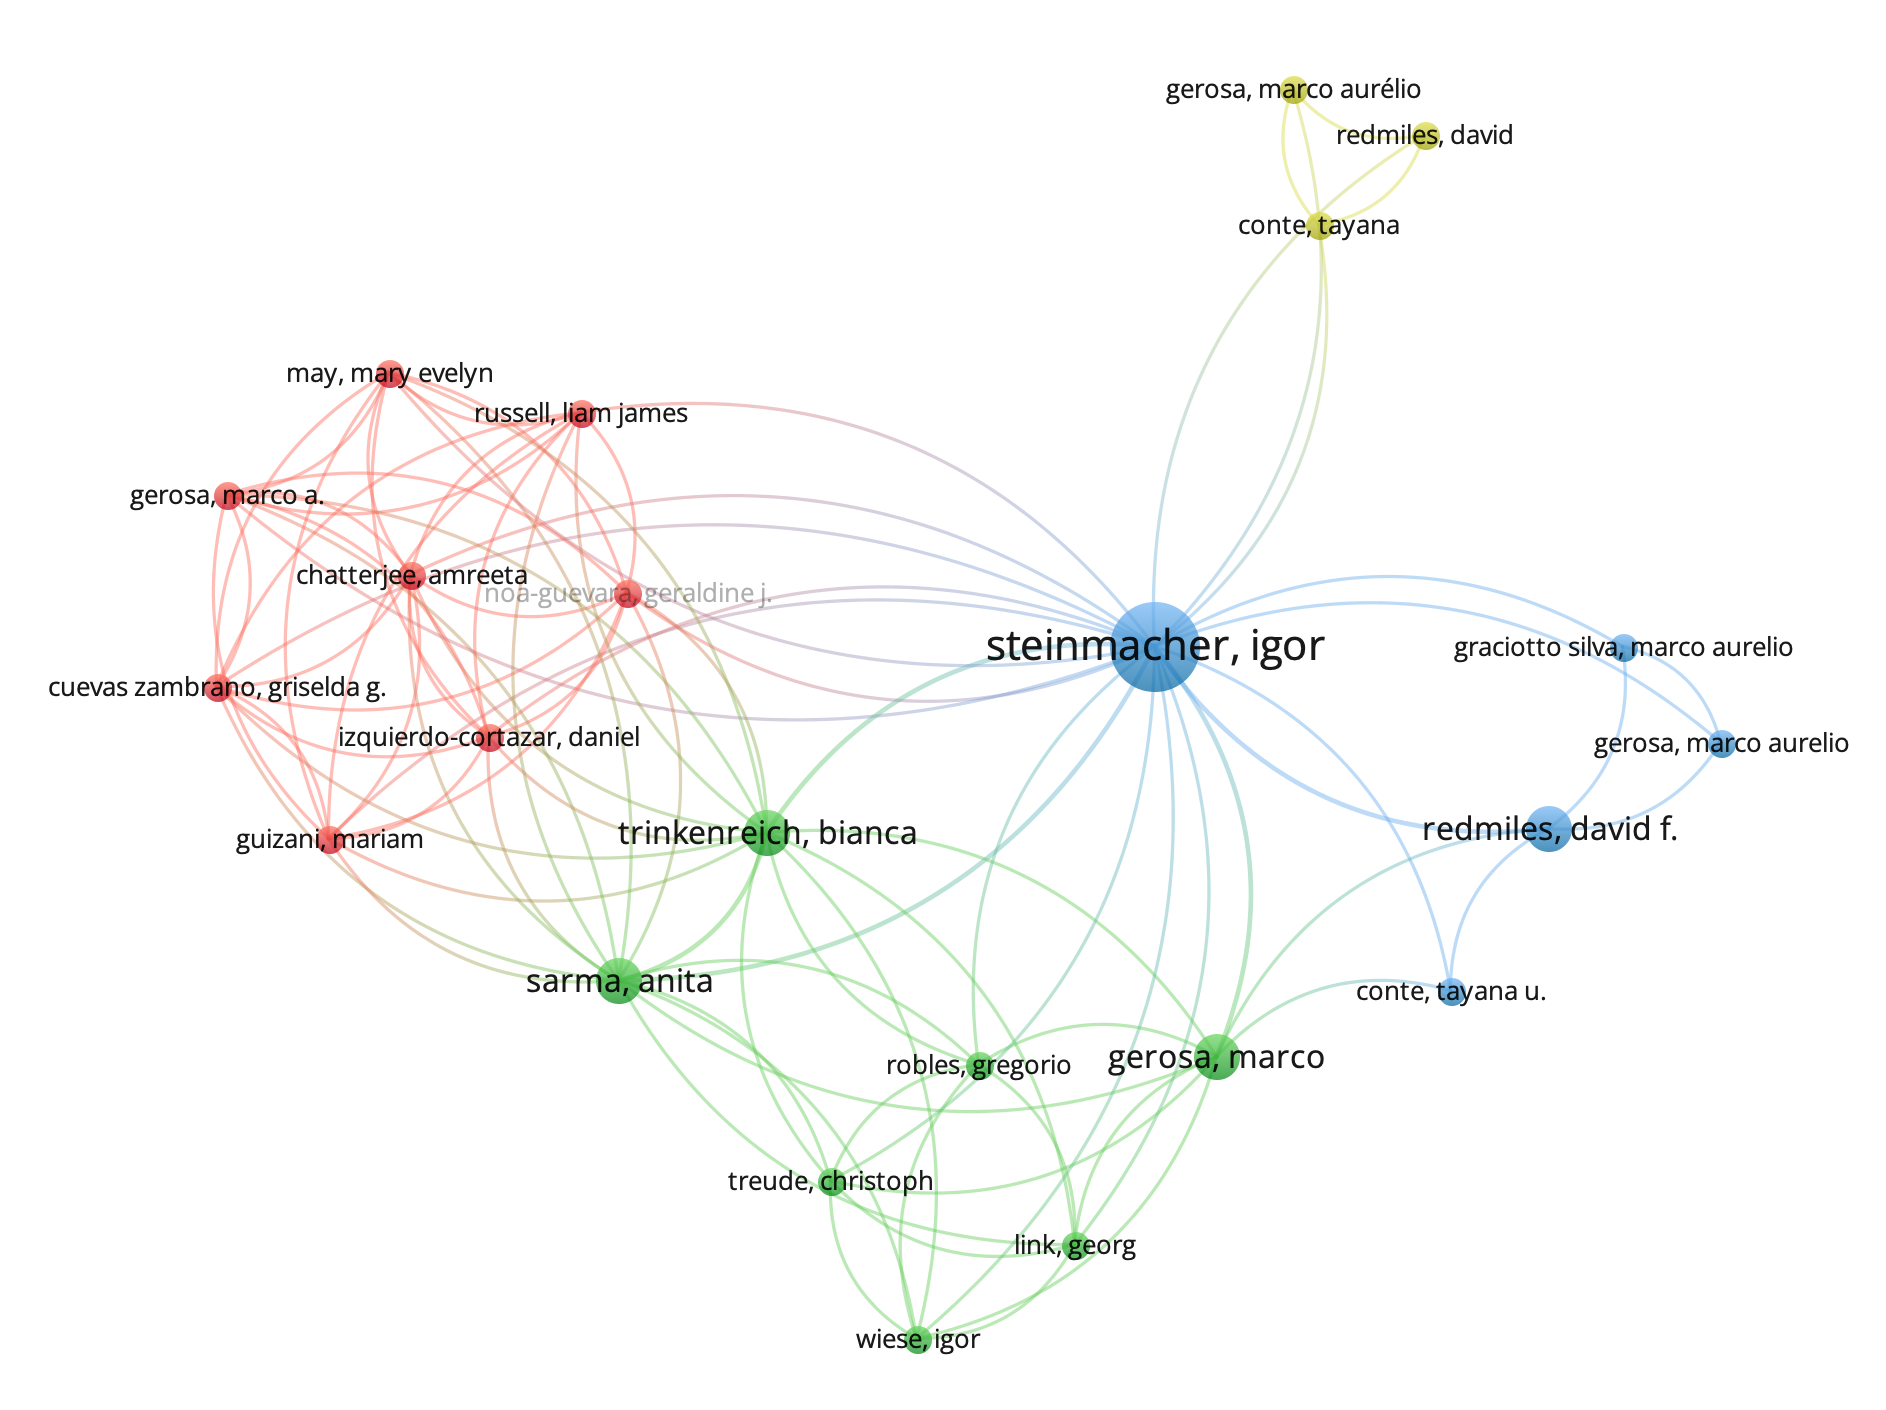
\includegraphics[width=1.1\linewidth]{figs/paperRelation.png}
    \caption{Collaboration relationship between authors of selected papers for SLR}
    \label{fig:paperRelation}
\end{figure}

The figure \ref{fig:paperRelation} depicts the collaboration network between authors of 20 selected papers for a systematic literature review on open-source software motivation, social impact, and challenges. The circles represent authors, and the connecting lines indicate co-authorship on a paper. The size of a circle corresponds to the number of papers an author has co-authored within the dataset. Steinmacher and Igor  appears to be the most prolific author in this dataset, having co-authored papers with several other researchers.

\subsection{Review conducting}

\subsubsection{Extract the data}
An essential stage in an SLR is data extraction. It entails the meticulous collection of precise and pertinent data from the research articles that I have selected for the review. Finding important data points that support the research questions is the first step in this procedure, which also involves methodically arranging the data to make analysis and synthesis of the results easier.
The information that will be taken from each paper is as follows:
\begin{itemize}
    \item Title
    \item Abstract
    \item Authors
    \item Publication date
    \item Database
    \item Keyword
    \item Research method
    \item Data collection method
    \item Answers to research questions
    \item Conclusion
\end{itemize}

\subsubsection{Synthesis}

To systematically analyze the extracted data, I formed two distinct groups (see Table \ref{tab:rq_articleId}) based on their focus:

\begin{itemize}
    \item Group 1: addressing interrelated research questions: This group delves into both research questions 1 and 2. Interestingly, a significant portion of papers addressing question 1 also provide answers to question 2. This overlap suggests a potential relationship between these two research questions. Group 1 comprises a total of 12 carefully selected papers.
    \item Group 2: exclusive focus on research question 3: This group offers a concentrated exploration of research question 3, without addressing the other research areas. Group 2 contains a total of 5 papers, ensuring a targeted examination of this specific question.
\end{itemize}


\begin{table}[ht]
    \centering
    \begin{tabular}{ | c | l |}
        \hline
        Research question & Article ID                                                   \\ \hline
        1                 & A05, A06 , A08 , A09, A10, A11, A12, A13, A15, A16, A17, A18 \\  \hline
        2                 & A05, A06, A07, A09, A10, A12, A13, A16, A17, A18, A19, A20   \\ \hline
        3                 & A01, A02, A03, A04, A14                                      \\ \hline
    \end{tabular}
    \caption{Data synthesis}
    \label{tab:rq_articleId}
\end{table}








\clearpage  % This command will start the next section from the new page
